\chapter{Introduction}
\label{ch:introduction}

\section{Motivation}
  Recent interest in advanced and next-generation nuclear power reactor designs
  has renewed the development of simulations for these reactors. A class of
  advanced nuclear power reactors which has merited research since the dawn of
  nuclear engineering is the Sodium-cooled Fast Reactor (SFR) which operates 
  with liquid sodium coolant and uses high-energy (``fast'') neutrons in the
  fission reaction. Since early development of SFRs such as the Experimental
  Breeder Reactor I (EBR-I) in 1951 and Fermi 1 in 1956, there have been
  significant innovations in both nuclear modeling and computational methods. As
  development of SFRs is revisited in the form of the Versatile Test Reactor
  (VTR) at Idaho National Laboratory (INL), these innovations in simulation can
  be used to simulate SFRs with modern best practices.
  Though this discussion has focused on reactors designed with sodium coolant,
  these methods can easily be used for reactors with lead or molten salt
  coolant.

  Nuclear reactor simulations are inherently multi-physics simulations. For
  example, neutron reaction probabilities are described by cross-sections.
  Neutron cross-sections are dependent on material temperatures and densities,
  both of which vary over the operating range of a nuclear power reactor. As
  reactor power changes, material temperatures and densities change, therefore
  cross-sections change and affect the reactor power. The multi-physics nature
  of the reactor necessitate a simulation of the power distribution within the
  reactor as well as all physical effects which will be modeled. In this
  application, the neutron diffusion equation is used to describe the reactor
  power distribution as in \chref{ch:neutronDiffusion}. Multi-physics effects
  are described by heat conduction and heat convection models as in
  \chref{ch:thermalHydraulics} as well as a thermal expansion model as in
  \chref{ch:thermalExpansion}.

  Ultimately, this simulation will model the steady-state behavior of SFRs using
  modern methods. By employing a modern solution method to the neutron diffusion
  equation in the form of the Finite Element Method (FEM), the simulation can
  take advantage of developments in numerical methods including the solution of
  linear systems. Additionally, the simulation allows for the incorporation of
  generalized multi-physics effects whereas current state-of-the-art simulations
  require data processing and manual calculation of multi-physics effects. The
  final simulation is designed to simulate an operating SFR.

\section{Geometry Description}
  \label{sec:geometry_description}
  Operating with fast neutrons decreases reaction probabilities. To compensate
  for this fact, SFRs are typically designed with hexagonal,
  triangularly-pitched, fuel assemblies to maximize the fuel packing and
  increase the fuel-density. An example of a SFR with hexagonal geometry as
  simulated in this method is given in \fref{fig:reactor_materials}.
  The specification of this geometry is necessary to
  describe material properties in the form of cross-sections as well as to
  describe coolant flow geometries. Dimensions of assemblies are measured at
  room temperature and will later be expanded according to the thermal expansion
  model.
  
  \begin{figure}
    \centering
    \includegraphics[width=\textwidth]{reactor_materials}
    \caption{Example of Sodium-cooled Fast Reactor based on MONJU.}
    \label{fig:reactor_materials}
  \end{figure}

  \begin{figure}
    \centering
    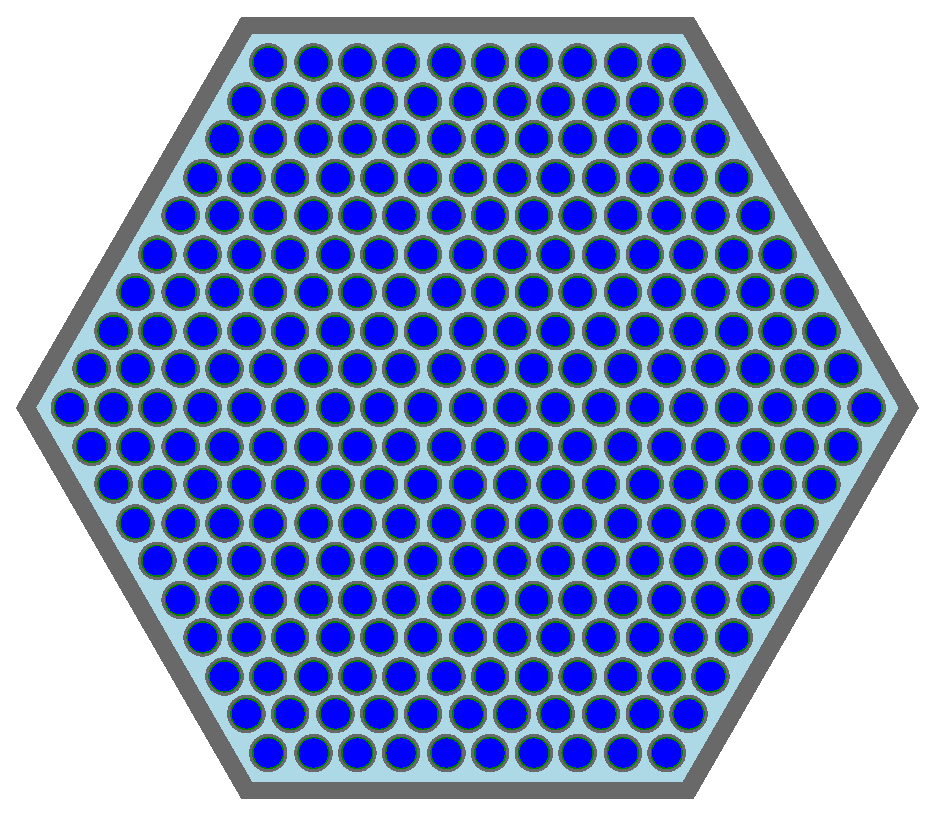
\includegraphics[width=0.5\textwidth]{prism_hex}
    \caption{Example of Sodium-cooled Fast Reactor Fuel Assembly.}
    \label{fig:prism_hex}
  \end{figure}

  In a cross section of a hexagonal assembly, dimensions are presented in
  A cross-sectional view of a single SFR fuel assembly is shown in 
  \fref{fig:prism_hex}. 
  Note the individual material pins are cylindrical and are then accumulated
  into a hexagonal assembly. The basic geometry is a fuel material within
  stainless steel cladding. The gap between the fuel and cladding is filled by
  sodium bond to improve thermal conductivity across the gap. Then the pin is
  wrapped by a steel wire to ensure separation between pins that will allow for
  coolant flow. The wire wrap also serves to encourage the mixture of coolant
  within the assembly. Many pins are then assembled into an assembly and
  surrounded by a hexagonal can made of steel. This can aids in structural
  stability and prohibits cross-flow between assemblies. 

  The dimensions within a single pin is shown in \fref{fig:pin_model} and the
  dimensions within a hexagonal assembly can is shown in \fref{fig:hex_can}. In
  \fref{fig:hex_can}, $T\!h_{Box}$ is the thickness of the assembly box,
  $F\!2\!F$ is the flat-to-flat measurement of the outside of the hexagonal can,
  and Pitch is the distance between the center of two pins. In future notation,
  the quantity ``Pitch'' is also denoted $S$. Using the geometry described in 
  these figures, the material cross-sectional areas are calculated according to 
  the given formulae where $N_{pin}$ is the number of pins in the assembly.
  \begin{align}
    \label{eq:afrac_first}
    A_{total} &= \frac{\sqrt{3}}{2} F\!2\!F^2 \\
    A_{can} &= A_{total} - 
      \frac{\sqrt{3}}{2} \left(  F\!2\!F - 2 \, T\!h_{Box} \right) \\
    A_{wrap} &= N_{pin} \frac{\pi}{4} D_{wrap}^2 \\
    A_{clad} &= N_{pin} \pi (R_C^2 - R_B^2) \\
    A_{bond} &= N_{pin} \pi (R_B^2 - R_F^2) \\
    A_{fuel} &= N_{pin} \pi R_F^2 \\
    \label{eq:afrac_last}
    A_{cool} &= A_{total} - A_{can} - A_{wrap} - A_{clad} - A_{bond} - A_{fuel}
  \end{align}
  Calculating the areas as above allows for calculation of cross-sectional area
  fractions. Assuming constant dimensions in the axial
  direction, these area fractions are equivalent to volume fractions and are
  useful for neutron cross-section calculations. Additionally, these formulae
  allow for thermal expansion calculations as the liquid sodium in the bond and
  the coolant are allowed to vary to allow for the expansion of other materials.

  \begin{figure}
    \centering
    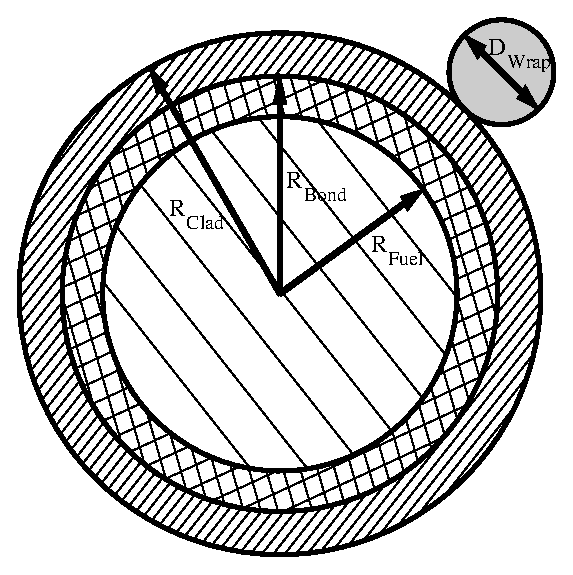
\includegraphics[width=0.5\textwidth]{pin_model}
    \caption{Dimensions of Thermal Hydraulic Pin Model.}
    \label{fig:pin_model}
  \end{figure}

  \begin{figure}
    \centering
    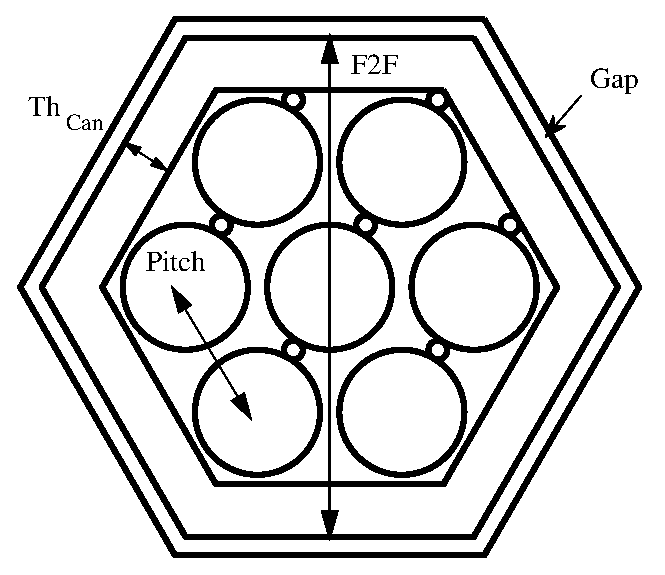
\includegraphics[width=0.5\textwidth]{hex_can}
    \caption{Dimensions of Hexagonal Can.}
    \label{fig:hex_can}
  \end{figure}

\section{Cross-Section Generation}
  Realistic cross-sections are pivotal to a realistic reactor simulation. There
  are two basic parts to cross-section treatment. First is the generation of
  cross-section libraries. The key to generating these libraries is using a
  representative flux spectrum for the many-group to multigroup collapse. It is
  impossible to know the exact spectrum at the time of library generation so an
  approximation decision must be made.
  For fissile compositions, the spectrum is given by the
  fission spectrum of the composition in some simplified geometry. For 
  non-fissile compositions, a flux spectrum and simplified geometry must be 
  assumed.  Using these flux spectra, the libraries must be generated at 
  selected temperatures to capture the effects of Doppler broadening.

  \subsection{Cross Section Library Generation}
    State-of-the-art fast reactor simulations utilize cross-sections generated
    from \mcc. This code from Argonne National Laboratory (ANL) allows for the
    generation of mulitgroup constants useful for solution of the neutron
    diffusion equation. The calculation in \mcc begins with a 2,082 fine-group
    neutron library based on ENDF-VII data and can be collapsed to an
    arbitrary, user-specified, energy group structure. For this application, the
    recommended and default 33-group structure is used. In fissile media, the
    energy spectrum used for the collapse is based on the fission spectrum of
    the media. In non-fissile media, a default \isotope[238]{U} fission spectrum
    is used \cite{mcc}.
    
    The collapse simplifies the geometry to an infinite and homogeneous medium.
    To reasonably simulate the energy spectrum within a hexagonal assembly,
    cross-sections are collapsed assuming an infinite homogeneous mixture 
    composed of a single hexagonal assembly. Number densities are calculated 
    such that the number density in the assembly is the number density within
    the material region weighted by the area fraction of that region. Area
    fractions are calculated by using \eref{eq:afrac_first} through 
    \eref{eq:afrac_last}.
    
    To capture the effect of Doppler broadening, cross-section libraries are
    generated for several different material temperatures.
    It is known that the effect of temperature on cross-sections are most
    significant in the fuel region where temperatures can be extreme at high
    reactor powers. Compared to the fuel temperature, the coolant and cladding
    temperatures change relatively little over the operating range of a
    sodium-cooled fast reactor.
    While fuel, clad, and coolant temperatures can be related as above (see
    \sref{sec:radial_conduction_model}), these
    relationships are functions of reactor power, $Q_{Rx}$, and reactor 
    coolant mass flow rate, $\mdot_{Rx}$, and these values are not known before 
    the simulation for a general reactor. Instead, a simplified temperature 
    relationship is used to generate the cross-section libraries.

    In each cross-section library, the coolant is maintained at some nominal
    temperature. For this application, that temperature is $400 \units{K}$
    (note: sodium melting temperature 371 \units{K}). Maintaining the coolant
    temperature as constant in this manner
    is acceptable because the dominant effect of temperature on the macroscopic
    cross-sections in the coolant is the density change of the fluid, not the
    Doppler effect. With constant coolant temperature, the fuel temperature is
    then varied over some range. For this application, libraries are generated
    for average fuel temperatures of 
    $400 \units{K}$, $600 \units{K}$, $900 \units{K}$, and $1200 \units{K}$. For
    each fuel temperature, the clad temperature is related as 
    \begin{equation}
      T_{clad} = \max \left\{ w \, T_{fuel}, T_{cool} \right\}
    \end{equation}
    % note: weight for T_{cool} should be 0.63 if perturbed coolant is desired
    where $w$ is a weighting factor, $T_{fuel}$ is the chosen fuel temperature
    for the library, and $T_{cool}$ is the chosen coolant temperature for the
    library. For this 
    application a weighting of $w=0.7$ provided acceptable results. This choice
    was based on analysis of the ratio $\overline{T_C}/\overline{T_F}$ for a
    representative high power reactor channel. Temperature
    in non-fissile assemblies is set to $T_{cool}$ during the collapse as there
    is no heat generated in these assemblies and in the steady-state axial
    convection model, non-fissile assemblies will have temperature equal to 
    $T_{inlet}$.

    \begin{table}
      \caption{Temperatures Selected for Cross-Section Libraries.}
      \label{tab:xstemps}
      \begin{center}
        \begin{tabular}{lll}
          \toprule
          $T_{cool} \units{K}$ & $T_{clad} \units{K}$ & $T_{fuel} \units{K}$ \\
          \midrule
          400 & 400 & 400  \\
          400 & 420 & 600  \\
          400 & 630 & 900  \\
          400 & 840 & 1200 \\
          \bottomrule
        \end{tabular}
      \end{center}
    \end{table}

    Ultimately, the cross-sections are accumulated as four separate libraries at
    temperatures given in \tref{tab:xstemps}. These cross-sections are generated
    at the temperatures specified and the collapses are performed assuming an
    infinite homogeneous mixture of a single assembly. With these libraries
    generated, the average material temperatures calculated in 
    \sref{sec:average_temps} are used to calculate cross-sections within each
    material using an interpolation method.

\section{Thesis Organization}
